% =====================================================================
%  BEST: a biological-fidelity framework for evaluating synthetic scRNA-seq
%  Application: NASA OSDR spaceflight transcriptomics (+ out-of-domain cancer control)
%  Target venue: npj Microgravity (Nature Portfolio)
%
%  REORGANIZED DRAFT (manuscript_reorg.tex). Full scholarly rewrite of
%  manuscript_filled.tex. Numbers are unchanged (from metrics_summary.csv);
%  figures (fig_*.pdf) are reused unchanged. Only writing, ordering, and
%  framing have changed.
% =====================================================================
\documentclass[11pt]{article}

\usepackage[utf8]{inputenc}
\usepackage[T1]{fontenc}
\usepackage[margin=1in]{geometry}
\usepackage{amsmath,amssymb}
\usepackage{graphicx}
\usepackage{xcolor}
\usepackage{booktabs}
\usepackage{array}
\usepackage{multirow}
\usepackage{caption}
\usepackage{authblk}
\usepackage{placeins}
\usepackage{tikz}
\usetikzlibrary{positioning,arrows.meta,fit,backgrounds}
\usepackage[hidelinks]{hyperref}

% ---- Editable handles -------------------------------------------------
% Framework name is wired through these two macros; change here to rename globally.
\newcommand{\fides}{BEST}
\newcommand{\protname}{BEST framework}
\newcommand{\Protname}{BEST framework}
\newcommand{\res}[1]{\textcolor{red}{[#1]}}
\newcommand{\figplaceholder}[2]{%
  \fbox{\begin{minipage}[c][#1][c]{0.92\linewidth}\centering
  \color{gray}\itshape #2\end{minipage}}}
% -----------------------------------------------------------------------

\captionsetup{font=small,labelfont=bf}
\setlength{\parskip}{4pt}

\title{\bfseries \fides{}: a biological-fidelity framework for evaluating synthetic single-cell RNA-seq, applied to spaceflight transcriptomics}

\author[1,2]{Arsh Suri\thanks{Corresponding author: suriarsh@gmail.com}}
\author[3]{Walter Alvarado}
\author[4]{James Casaletto}
\affil[1]{Wallace H.\ Coulter Department of Biomedical Engineering, Georgia Institute of Technology, Atlanta, GA, USA}
\affil[2]{Space Life Sciences Training Program, NASA Ames Research Center, Moffett Field, CA, USA}
\affil[3]{Space Biosciences Research Branch, NASA Ames Research Center, Moffett Field, CA, USA}
\affil[4]{Blue Marble Space Institute of Science, Seattle, WA, USA}

\date{}

\begin{document}
\maketitle

% =====================================================================
\begin{abstract}
\noindent
Spaceflight reshapes the transcriptome, yet the cohorts available to study it are among the smallest in modern genomics, which limits statistical power and the development of predictive models for astronaut health. Deep generative models can augment these scarce single-cell RNA sequencing (scRNA-seq) datasets, but synthetic single-cell data is judged almost entirely by distributional metrics that are blind to biology, so a generator can satisfy them while discarding the very signal a dataset exists to carry. We present \fides{} (Biological Evaluation of Synthetic Transcriptomics), a biological-fidelity evaluation framework that governs every comparison by a single principle: derive a biological quantity from synthetic data and score it against the same quantity derived from real held-out data. \fides{} trains and stops every generator at a common distributional operating point using an MMD criterion in a frozen principal-component space, then evaluates a statistical-distance layer (Layer~0; distributional distances such as Wasserstein and Mahalanobis) together with three biological layers that distributional metrics miss: overlap of the top differentially expressed genes for a condition contrast (Layer~1), overlap of the genes a classifier finds most predictive of that contrast (Layer~2), and overlap of the gene-ontology terms enriched among those predictive genes (Layer~3). \fides{} is delivered as a scalable, model-agnostic pipeline with built-in training and stopping, so any group can generate a conditioned one-to-one replicate of a dataset and benchmark competing generators' biological fidelity on equal terms. We exercise the framework with three generators spanning the main families of deep generative modeling: a conditional variational autoencoder, the classifier-free latent diffusion model cfDiffusion, and a multi-conditional adaptation of scGAN, each conditioned on an identical five-attribute covariate vector and each stopped at a common distributional operating point so that the biological comparison reflects the generated data rather than unequal training. Across five spaceflight configurations from the NASA Open Science Data Repository (OSDR) and an out-of-domain colorectal-cancer control, the biological layers separate models that converge to a similar distributional operating point, pathway-level fidelity can exceed gene-level fidelity, and the architectures diverge sharply in how well they preserve single-cell sparsity. This provides the first multi-conditional application of GAN and diffusion generative models, with biology-aware evaluation, to spaceflight single-cell transcriptomics.
\end{abstract}

% =====================================================================
\section{Introduction}

\subsection{Spaceflight remodels the transcriptome under constrained sampling}
Extended spaceflight alters human physiology through stressors absent from terrestrial evolution. Astronauts experience roughly 1.5\% monthly bone loss, cardiovascular deconditioning, and immune dysfunction, and these changes are accompanied by extensive transcriptomic reprogramming \cite{twins}. The NASA Twins Study found that over one thousand genes showed expression or epigenetic changes during flight, most returning toward baseline within six months while a subset governing DNA repair, immune response, and bone formation remained altered \cite{twins}. The Inspiration4 mission and subsequent multi-omic atlases identified a recurring spaceflight signature spanning oxidative phosphorylation, immune function, and stress-response programs \cite{i4}. Single-cell resolution is increasingly central to resolving which cell populations drive these responses, but spaceflight single-cell datasets remain rare and small.

\subsection{Data scarcity constrains spaceflight omics}
Fewer than six hundred people have flown in space, individual studies typically involve fewer than twenty subjects, and rodent missions are similarly limited once samples are stratified by tissue, sex, age, and mission \cite{ilangovan,scott}. The NASA Open Science Data Repository (OSDR) aggregates hundreds of transcriptomic datasets, yet small per-study sizes and preservation-related batch effects can eclipse the spaceflight signal itself \cite{osdr}. Prior NASA analyses have explicitly identified sample-power limitation as the central obstacle to applying machine learning in this domain and have called for methods that cope with extreme sample scarcity \cite{scott,ilangovan}. Synthetic data augmentation is the standard remedy for this regime.

\subsection{Synthetic scRNA-seq evaluation ignores biology}
Deep generative models for scRNA-seq now span variational autoencoders \cite{scvi,activa}, generative adversarial networks \cite{scgan}, and diffusion and flow-matching models \cite{scdiffusion,cfdiffusion,cfgen}, alongside analytical simulators \cite{scgft,scdesign3,simbench}. Yet these models are compared almost exclusively through distributional similarity, for example maximum mean discrepancy (MMD), Fr\'echet-style distances, or a classifier two-sample test in which chance-level discrimination signals success \cite{scgan,scdiffusion}. Such metrics can be satisfied by data that is statistically plausible yet biologically hollow, preserving marginal distributions while losing the condition contrasts, mechanistic pathways, and predictive gene programs that make a dataset useful for discovery. No widely used benchmark asks whether a synthetic dataset reproduces the differential expression, the predictive gene programs, or the enriched biology of the data it imitates.

\subsection{Deep learning has barely reached spaceflight single-cell data}
Generative modeling of spaceflight transcriptomes has so far been confined almost entirely to bulk RNA-seq, most notably with generative adversarial networks for OSDR biomarker discovery \cite{ganbio}, alongside a conference-only poster that applied a conditional variational autoencoder (CVAE) to spaceflight single-nucleus RNA-seq from our group \cite{ntrs} and a recent augmentation framework for spaceflight omics \cite{glare}. GAN and diffusion models, which dominate generative modeling elsewhere, have not been brought to spaceflight single-cell data, and none of this prior work couples a multi-conditional, multi-architecture single-cell generator to a biology-aware evaluation.

\subsection{Contributions}
This work makes two coupled contributions.

\noindent\textbf{A biological-fidelity evaluation framework (\fides{}).} We introduce a uniform, biology-aware evaluation of synthetic scRNA-seq with two inseparable facets. The first is a set of biology-aware metrics absent from current practice: alongside a statistical-distance layer (Layer~0; Wasserstein, Mahalanobis, and related distributional distances) and an MMD-based training and stopping rule, \fides{} scores the overlap of the top differentially expressed genes for a condition contrast (Layer~1), the overlap of the genes a classifier finds most predictive of that contrast (Layer~2), and the overlap of the gene-ontology terms enriched among those predictive genes (Layer~3). Together these ask whether synthetic data preserves the experimental contrast, the predictive gene programs, and the mechanisms that give the contrast meaning. The predictive-gene enrichment layer is, to our knowledge, new to synthetic-data evaluation. The second facet is the delivery: \fides{} is a scalable, model-agnostic pipeline with built-in training and stopping that any group can run on any scRNA-seq dataset with any generator, holding every generator to a common MMD-based operating point and retaining the Layer~0 statistical distances so that runs stay comparable, and making model-versus-model biological benchmarking straightforward. The accessibility of the pipeline and the ease of fair biological comparison it provides are themselves core contributions, not packaging.

\noindent\textbf{Multi-conditional GAN and diffusion generation for spaceflight single-cell transcriptomics.} We adapt two deep generative architectures to condition jointly on the full set of mission covariates and apply them, for the first time, to NASA OSDR spaceflight scRNA-seq, the domain where sample-power limitation is most acute \cite{scott,ilangovan}. The classifier-free latent diffusion model cfDiffusion \cite{cfdiffusion} and scGAN \cite{scgan} were originally conditioned on a single attribute; we extend both to accept an identical five-attribute covariate vector (experimental condition, strain, sex, age at launch, and mission duration), so that condition-controllable in silico cohorts can be generated across genetic backgrounds, sexes, and ages. This multi-conditional capability enables the in silico cohorts that spaceflight medicine needs and, together with a CVAE, provides a testbed that spans the main families of deep generative modeling. The generators are existing, published methods used to exercise \fides{}; the contribution is the evaluation and its first multi-conditional application to this domain, not a new generator, and we neither crown a best model nor treat the architectural extension as a modeling advance in itself. Where one architecture leads on biological fidelity we report it as a scoping observation, not a general ranking, since recent evidence on synthetic scRNA-seq is mixed \cite{cfgen,scgft,scdiffusion}.

% =====================================================================
\section{Results}

\subsection{\fides{}: a layered, biology-aware evaluation framework}
\fides{} evaluates synthetic scRNA-seq through one governing design, which we denote train-on-synthetic, test-on-real (TSTR): every quantity of interest is derived from synthetic data and scored against the same quantity derived from real held-out data. Before evaluation, the pipeline trains and stops every generator at a common distributional operating point using an MMD criterion computed in a frozen 50-component principal-component space, so that runs remain comparable across models and datasets; this training and stopping stage is distinct from the evaluation layers below. The framework then evaluates four layers (Fig.~\ref{fig:framework}): a statistical-distance layer (Layer~0; distributional distances such as Wasserstein, Mahalanobis, cosine, and mean absolute deviation) and three biological layers that ask, in sequence, whether the synthetic data preserves the experimental contrast (Layer~1, differential expression), the predictive gene programs (Layer~2, phenotype classification), and the mechanisms behind them (Layer~3, enrichment of the predictive genes). Layer~3 consumes Layer~2's gene list directly, so the mechanistic test is tied to the predictive one rather than computed on an unrelated set.

A single binary phenotype contrast defines all three biological layers: the two classes are simultaneously the groups compared for differential expression, the labels the classifier is trained to separate, and the basis for the enriched-gene analysis. For the OSDR datasets this contrast is spaceflight versus ground control; for the cancer control it is metastatic-site tumor versus adjacent normal tissue. Fixing one contrast across the layers makes the three biological scores directly comparable and ensures they interrogate the same biology.

Throughout, we use \emph{fidelity} to mean how faithfully the synthetic data reproduces a specific biological property of the real data, and we report each biological layer as a single, directly comparable percentage computed on held-out test cells. For the two gene-list layers (condition and phenotypic fidelity), the overlap percentage is the number of genes common to the real and synthetic top-50 lists divided by 50, so 100\% means the ranked lists are identical and 0\% means they are disjoint. For the mechanistic layer, the percentage is the fraction of the real data's significantly enriched gene-ontology terms that are also enriched among the synthetic data's predictive genes. Higher is better for all three; the statistical measures (the Layer~0 distances and the MMD training operating point) instead report distances, for which lower is better.

To exercise \fides{} we generated synthetic data with three established generators that span the main families of deep generative modeling: a CVAE, the classifier-free latent diffusion model cfDiffusion \cite{cfdiffusion}, and a multi-conditional adaptation of scGAN \cite{scgan}. These are existing methods used as a testbed; our purpose is to evaluate the data they produce, not to introduce or crown a generator. All three were trained on identical inputs, conditioned on an identical five-attribute covariate vector, and stopped at a common distributional operating point, so that any difference the biological layers report reflects the fidelity of the generated data rather than unequal training (Methods).

\begin{figure}[t]
\centering
\resizebox{\textwidth}{!}{%
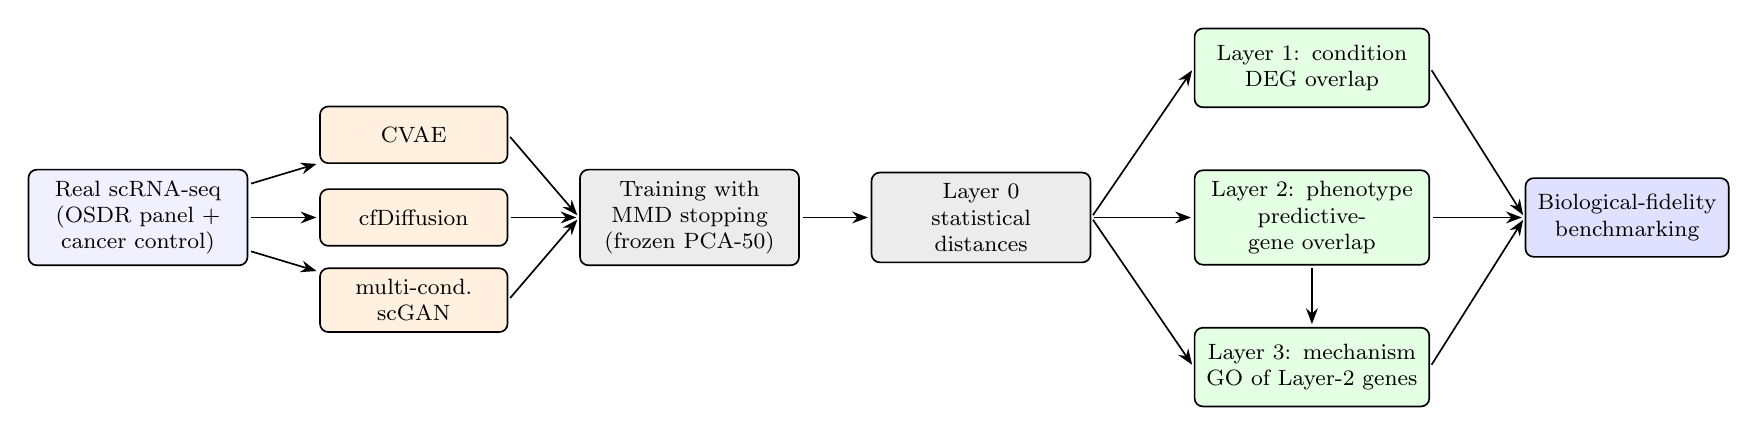
\begin{tikzpicture}[
  font=\footnotesize,
  >={Stealth[]}, semithick,
  base/.style={draw, rounded corners=3pt, align=center, inner sep=4pt, minimum height=1.0cm, text width=2.5cm},
  data/.style={base, fill=blue!6},
  model/.style={base, fill=orange!12, minimum height=0.72cm, text width=2.1cm},
  proc/.style={base, fill=gray!15},
  bio/.style={base, fill=green!10, text width=2.7cm},
  score/.style={base, fill=blue!12, text width=2.3cm},
  arr/.style={->, shorten >=1pt, shorten <=1pt}
]
\node[data] (data) {Real scRNA-seq\\(OSDR panel +\\cancer control)};
\node[model, right=0.9cm of data, yshift=1.05cm] (cvae) {CVAE};
\node[model, right=0.9cm of data] (diff) {cfDiffusion};
\node[model, right=0.9cm of data, yshift=-1.05cm] (gan) {multi-cond.\ scGAN};
\node[proc, right=0.9cm of diff] (train) {Training with\\MMD stopping\\(frozen PCA-50)};
\node[proc, right=0.9cm of train] (l0) {Layer 0\\statistical\\distances};
\node[bio, right=1.3cm of l0, yshift=1.9cm] (l1) {Layer 1: condition\\DEG overlap};
\node[bio, right=1.3cm of l0] (l2) {Layer 2: phenotype\\predictive-gene overlap};
\node[bio, right=1.3cm of l0, yshift=-1.9cm] (l3) {Layer 3: mechanism\\GO of Layer-2 genes};
\node[score, right=1.2cm of l2] (score) {Biological-fidelity\\benchmarking};

\draw[arr] (data) -- (cvae);
\draw[arr] (data) -- (diff);
\draw[arr] (data) -- (gan);
\draw[arr] (cvae.east) -- (train.west);
\draw[arr] (diff.east) -- (train.west);
\draw[arr] (gan.east) -- (train.west);
\draw[arr] (train) -- (l0);
\draw[arr] (l0.east) -- (l1.west);
\draw[arr] (l0.east) -- (l2.west);
\draw[arr] (l0.east) -- (l3.west);
\draw[arr] (l2) -- (l3);
\draw[arr] (l1.east) -- (score.west);
\draw[arr] (l2.east) -- (score.west);
\draw[arr] (l3.east) -- (score.west);
\end{tikzpicture}}
\caption{\textbf{The \fides{} framework and its multi-model testbed.} Three representative generators are trained on identical inputs with an identical five-attribute conditioning vector and stopped at a common distributional operating point by a shared MMD rule computed in a frozen 50-component PCA space; this training and stopping stage is upstream of evaluation and is what makes the generators comparable. Generated data then passes a statistical-distance layer (Layer~0, distributional distances such as Wasserstein and Mahalanobis), from which three biology-aware layers branch under a train-on-synthetic, test-on-real design: condition preservation (Layer~1, top-50 differentially expressed gene overlap), phenotypic preservation (Layer~2, random-forest predictive-gene overlap), and mechanistic preservation (Layer~3, gene-ontology enrichment of the Layer-2 predictive genes). The pipeline is architecture- and dataset-agnostic and is built so that any group can run it and compare generators' biological fidelity on equal terms.}
\label{fig:framework}
\end{figure}

\subsection{An MMD rule gives an architecture-agnostic stopping point}
Loss values are not comparable across architectures: the CVAE optimizes an evidence lower bound, scGAN optimizes an adversarial Wasserstein objective whose magnitude is unbounded and does not track sample quality, and the diffusion model optimizes a denoising loss. Stopping each model on its own loss would compare the three at incommensurable operating points. We therefore stopped every model on the same external criterion, MMD between real and synthetic data measured in a frozen 50-component principal-component space, and halted when it ceased to improve (Fig.~\ref{fig:mmd}; Methods). The multi-conditional scGAN reached the lowest converged MMD on every dataset (0.049 to 0.155), the CVAE was intermediate, and cfDiffusion was generally highest (up to 0.735). Because the three nonetheless diverge on the biological layers below, this operating point is a fair common stopping rule, not a ranking of biological quality: MMD convergence certifies comparable distributional quality, not that the biology has been learned.

\begin{figure}[ht]
\centering
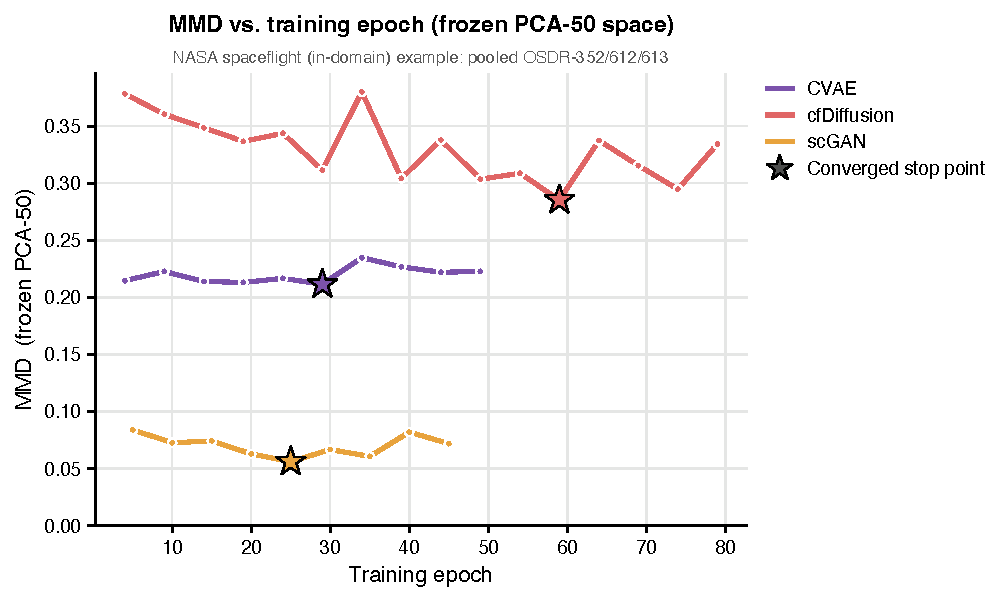
\includegraphics[width=0.78\linewidth]{fig_mmd_convergence.pdf}
\caption{\textbf{MMD-based training and stopping.} Maximum mean discrepancy between real and synthetic data, computed in a frozen 50-component PCA space, as a function of training epoch for the CVAE, cfDiffusion, and multi-conditional scGAN on a representative dataset (pooled OSDR-352/612/613). A fixed real reference sample is compared against a freshly generated synthetic sample at each evaluation; training halts when MMD ceases to improve. Stars mark each generator's converged operating point. scGAN reaches and holds the lowest MMD, cfDiffusion the highest, giving an architecture-agnostic operating point at which the models are compared.}
\label{fig:mmd}
\end{figure}
\FloatBarrier

\subsection{Layer 1, condition fidelity: differentially expressed gene overlap}
For each dataset we identified the top 50 genes distinguishing the phenotype contrast, ranked by absolute log fold change, separately in real and synthetic data, and measured the percentage of genes shared between the two lists (Methods). This asks whether the synthetic data preserves the biological contrast that motivates the experiment, a stronger test than overall distributional similarity. The multi-conditional scGAN led on five of the six datasets, reaching up to 36\% overlap on spaceflight data (pooled OSDR-352/612/613 and OSDR-404) and 56\% on the out-of-domain cancer control, while the CVAE and cfDiffusion were lower on the spaceflight studies, with cfDiffusion the exception on the pooled brain set (38\% versus scGAN's 36\%) (Fig.~\ref{fig:overlap}a; Table~\ref{tab:bio}). The choice of $N=50$ is a convention: the metric is defined for any top-$N$ list.

\begin{figure}[ht]
\centering
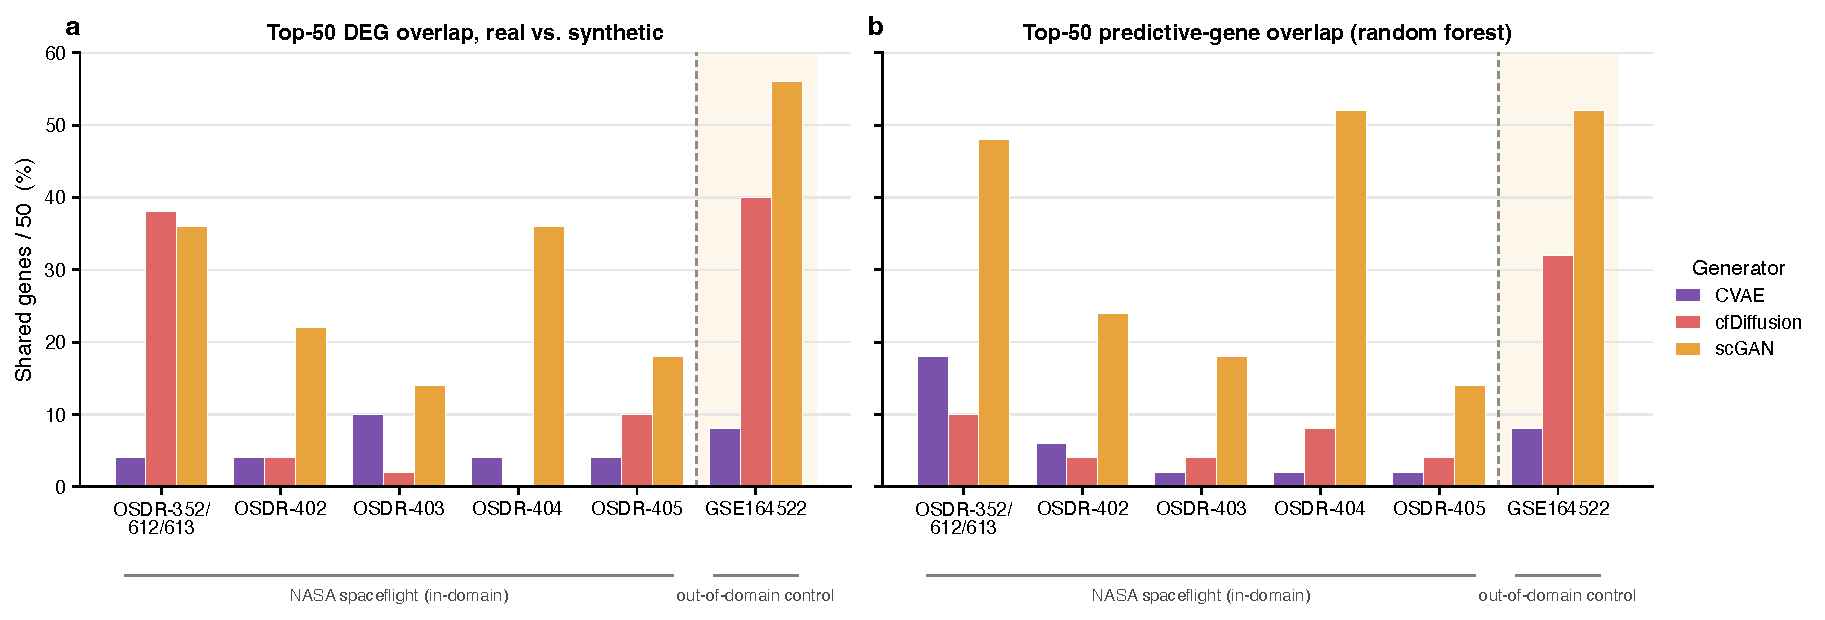
\includegraphics[width=\linewidth]{fig_overlap.pdf}
\caption{\textbf{Condition and phenotype fidelity across datasets.} Top-50 differentially expressed gene overlap (a, Layer~1) and random-forest predictive-gene overlap (b, Layer~2) between real and synthetic data, grouped by dataset and generator; the shaded column and bracket labels mark the out-of-domain cancer control against the in-domain spaceflight datasets. The multi-conditional scGAN leads on condition fidelity for five of six datasets and on phenotypic fidelity for all six, with the largest margins on the pooled brain set and the two largest datasets.}
\label{fig:overlap}
\end{figure}

\subsection{Layer 2, phenotypic fidelity: predictive-gene overlap under TSTR}
We next asked whether the synthetic data preserves the gene programs that are predictive of the phenotype. We trained random-forest classifiers to distinguish the contrast, one on synthetic data and one on real data, and compared their top-50 most important genes as the percentage shared (Methods). This is the canonical TSTR case and inverts the classifier two-sample test of prior work: there, chance-level discrimination between real and synthetic cells is the goal; here, high agreement between the real and synthetic classifiers' predictive genes is the goal. The multi-conditional scGAN led on every dataset, with feature-importance overlap reaching 52\% (OSDR-404 and the cancer control) and 48\% on the pooled brain set, whereas the CVAE and cfDiffusion remained at or below 18\% on all spaceflight studies (Fig.~\ref{fig:overlap}b; Table~\ref{tab:bio}).

The accuracy of these classifiers is a separate, secondary diagnostic. We report it in Table~\ref{tab:stat} as TSTR accuracy, the accuracy of the synthetic-trained classifier evaluated on real cells; it is not a synthetic-versus-real discrimination test, and it must be read against class imbalance. For the CVAE it dissociates cleanly from gene overlap: the CVAE reached high TSTR accuracy (0.93 on OSDR-402, 0.96 on the cancer control) while sharing only 6 to 8\% of important genes with the real classifier, a clear case in which surface accuracy does not imply that the synthetic data encodes the same mechanistic basis for the prediction. We therefore lead Layer~2 with feature-importance overlap and treat accuracy as secondary. The spaceflight contrasts carry majority-class baselines of 52.7 to 70.0\% (Table~\ref{tab:clf}), so a classifier can match the baseline while collapsing to the majority class, which the real and cfDiffusion classifiers do on OSDR-402, OSDR-404, and OSDR-405 (macro-F1 $\le 0.02$). Real-data classifiers reached 0.54 to 0.81 accuracy on the same contrasts, only $-0.1$ to $+20.1$ points above their majority baselines (Table~\ref{tab:clf}); the two large cohorts (pooled brain $+14.9$, cancer $+20.1$) are where the classification signal is genuinely earned rather than inherited from imbalance.

\FloatBarrier
\subsection{Layer 3, mechanistic fidelity: pathway enrichment of predictive genes}
Because two datasets can share biological function without sharing exact gene identities, we asked whether the predictive genes implicate the same biology. Using the \emph{same} top-50 random-forest genes that define Layer~2, we computed gene-ontology over-representation separately on the real and synthetic gene lists and measured, among the top ten enriched terms, the percentage of the real data's enriched terms that the synthetic data also recovers (Methods). Because the gene set is the classifier's own predictive genes, this layer tests whether a model's predictive signal rests on the same mechanisms as the real data, not merely on statistically similar genes.

Where recoverable signal existed, pathway overlap exceeded gene-level overlap. On the pooled OSDR-352/612/613 set all three generators recovered 8 to 9 of the 10 real pathways (80 to 90\%) against 4 to 38\% gene-level overlap (Fig.~\ref{fig:fgsea}; compare Fig.~\ref{fig:overlap}a). The recovered programs were biologically coherent. On OSDR-404 (blood) the real data was enriched for cytoplasmic translation and ribosomal structural pathways, and scGAN recovered seven of ten; on the cancer control the real data was enriched for T-cell and lymphocyte activation and immune-response pathways, and scGAN recovered eight of ten. The misses were equally informative: on OSDR-403 (bone marrow) the real data was enriched for tissue-appropriate B-cell differentiation and hematopoietic programs, yet no generator recovered any of them (0 of 10), and on OSDR-405 (spleen) only cfDiffusion recovered any pathways (20\%). These are recovery gaps rather than absent biological signal, and they localize precisely where each generator loses the biology. That a generator conditioned on five attributes at once can still recover 70 to 90\% of the real enriched programs on the larger cohorts shows that the multi-conditional adaptation preserves coordinated transcriptional programs, not just marginal gene statistics.

\begin{figure}[ht]
\centering
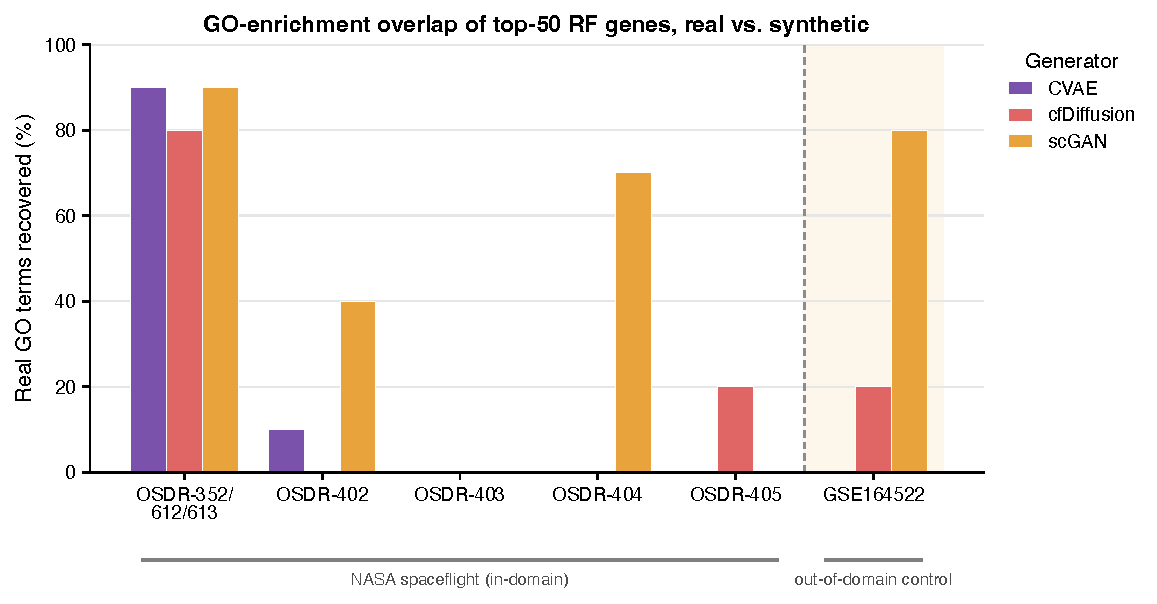
\includegraphics[width=0.82\linewidth]{fig_fgsea.pdf}
\caption{\textbf{Mechanistic fidelity: GO enrichment of the predictive genes (Layer~3).} Gene-ontology terms over-represented among each model's top-50 random-forest genes (hypergeometric test against MSigDB, top 10 per dataset, FDR $q<0.05$), reported as the percentage of the real data's enriched terms recovered in the synthetic data. Where recoverable signal exists, pathway overlap exceeds gene-level overlap (compare Fig.~\ref{fig:overlap}a): all three generators recover 80 to 90\% of pathways on the pooled brain set, and scGAN recovers 70\% on OSDR-404 and 80\% on the cancer control. Recovered programs are dominated by cytoplasmic translation and ribosomal pathways in spaceflight data and by lymphocyte and T-cell activation in the cancer control; OSDR-403 (bone marrow) shows the opposite case, where tissue-appropriate real enrichment is not recovered by any generator.}
\label{fig:fgsea}
\end{figure}

\subsection{A scalable, model-agnostic pipeline, robust out of domain}
\fides{} is built to run unchanged on any dataset and any generator. Applying the identical pipeline, with no retraining strategy, hyperparameter change, or metric modification, to the out-of-domain GSE164522 colorectal-cancer tumor-immune dataset (190{,}519 cells; metastatic-site tumor versus adjacent normal) reproduced the within-spaceflight behavior: scGAN again led on all three biological layers (56\% DEG, 52\% predictive-gene, and 80\% pathway overlap) and reached the lowest MMD, while preserving near-real sparsity (Tables~\ref{tab:stat},~\ref{tab:bio}). Across the panel the pipeline handled 1{,}534 to 213{,}854 cells and three architectures from three generative families on the same footing, with the common MMD operating point and the Layer~0 statistical distances retained so results stay comparable across runs. This is the practical contribution of the framework as much as the metrics are: it gives the field a single, low-friction way to compare the biological fidelity of competing generators on equal terms, rather than re-implementing an ad hoc evaluation for each new model.

\subsection{Biological fidelity scales with training-set size}
A clear trend runs across the panel: biological fidelity rises with the number of training cells (Fig.~\ref{fig:size}). The three smallest cohorts (OSDR-402, OSDR-403, and OSDR-405, each under 3{,}500 cells) are the weakest across all three biological layers, whereas the three largest (OSDR-404 at 14{,}045 cells and the two roughly 200{,}000-cell sets) are the strongest. For the multi-conditional scGAN, mean biological fidelity rises from about 11\% on the smallest studies to 53 to 63\% on the largest (Spearman $\rho=0.77$ against cell count; $\rho=0.89$ for cfDiffusion), and the two deep generators scale more steeply than the CVAE. This is the expected and sobering shape for the spaceflight regime: the smallest cohorts, which most need augmentation, are the hardest to reproduce faithfully, while fidelity improves markedly once a few tens of thousands of cells are available (OSDR-404, at 14{,}045 cells, already behaves like the largest sets). The modest overlaps on the smallest studies therefore reflect data scarcity rather than a ceiling of the framework or of the multi-conditional adaptation.

\begin{figure}[ht]
\centering
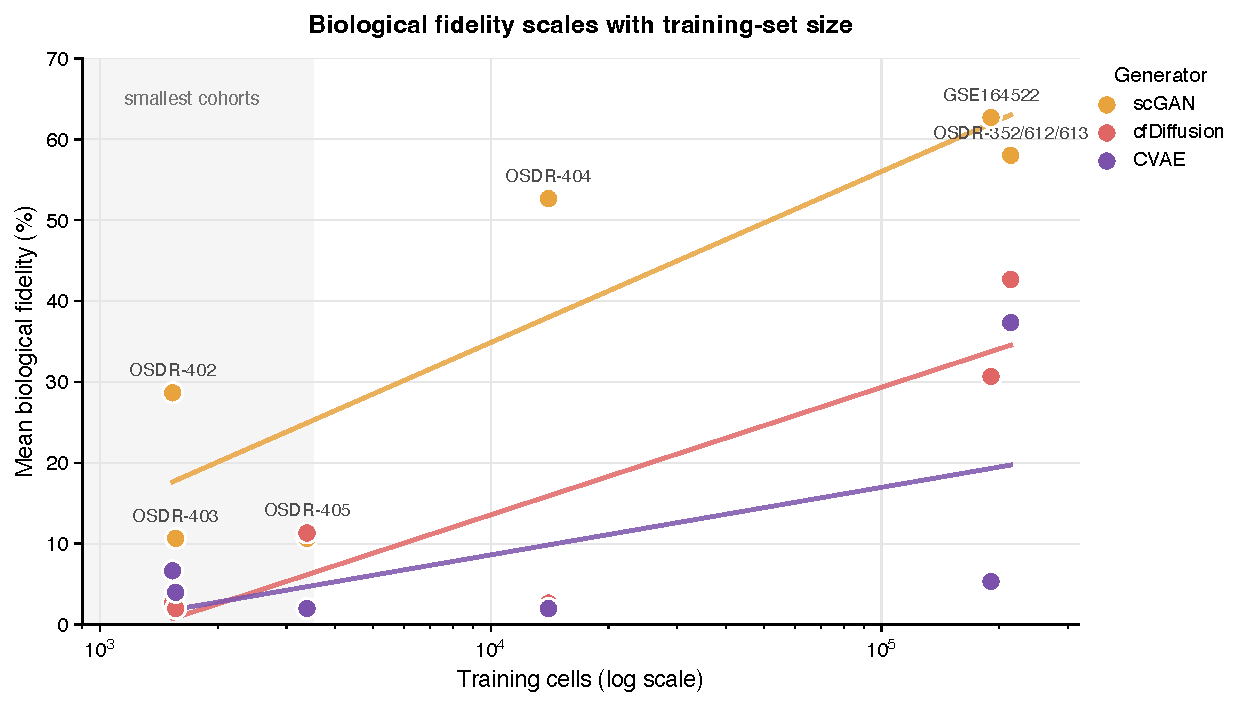
\includegraphics[width=0.78\linewidth]{fig_size_trend.pdf}
\caption{\textbf{Biological fidelity scales with training-set size.} Mean of the three biological-fidelity metrics (top-50 DEG overlap, predictive-gene overlap, and GO-enrichment overlap) per generator against the number of training cells (log scale); lines are least-squares fits in log-cell space. All generators improve with size and the two deep generators scale most steeply; the shaded band marks the smallest cohorts (under 3{,}500 cells).}
\label{fig:size}
\end{figure}

\begin{figure}[ht]
\centering
\figplaceholder{5.6cm}{Figure placeholder: UMAP embeddings. \\ Real versus synthetic cells for representative datasets, one panel per architecture, colored by condition and by data source (real vs.\ synthetic). UMAP was disabled in the reported pipeline run; this panel can be generated from the stored h5ad replicates if desired.}
% \includegraphics[width=0.85\linewidth]{fig_umap.pdf}
\caption{\textbf{Manifold overlap by architecture.} UMAP embeddings of real and synthetic cells for representative datasets. Columns correspond to the CVAE, cfDiffusion, and multi-conditional scGAN; points are colored by experimental condition and by real versus synthetic origin. \res{Placeholder: UMAP was disabled in the reported pipeline run; generate from stored h5ad replicates if desired.}}
\label{fig:umap}
\end{figure}

\FloatBarrier
% ---------- Summary tables (after the Results figures) ----------
\begin{table}[t]
\centering
\caption{\textbf{Dataset panel.} Five spaceflight configurations drawn from NASA OSDR, evaluated as individual Rodent Research Reference Mission-2 (RRRM-2) studies and as one pooled brain cohort, together with one out-of-domain cancer control. All spaceflight datasets contrast spaceflight versus ground control; the cancer control contrasts metastatic-site tumor versus adjacent normal tissue. Cell counts are the processed, HVG-selected matrices used for generation and evaluation.}
\label{tab:data}
\small
\resizebox{\textwidth}{!}{%
\begin{tabular}{@{}llrcl@{}}
\toprule
Dataset (label) & Domain / tissue & Cells & Contrast & Notes \\
\midrule
OSDR-352/612/613 (pooled) & Spaceflight, brain & 213{,}854 & Flight vs.\ Ground & Pooled across OSDR-352 / 612 / 613; 3 strains \\
OSDR-402 & Spaceflight, femur bone marrow & 1{,}534 & Flight vs.\ Ground & RRRM-2; C57BL/6NTac, female \\
OSDR-403 & Spaceflight, humerus bone marrow & 1{,}561 & Flight vs.\ Ground & RRRM-2; C57BL/6NTac, female \\
OSDR-404 & Spaceflight, PBMC (blood) & 14{,}045 & Flight vs.\ Ground & RRRM-2; C57BL/6NTac, female \\
OSDR-405 & Spaceflight, spleen & 3{,}384 & Flight vs.\ Ground & RRRM-2; C57BL/6NTac, female \\
GSE164522 (cancer) & Colorectal cancer, tumor-immune (10x) & 190{,}519 & Tumor vs.\ Normal & Out-of-domain control; liver-metastasis atlas \\
\bottomrule
\end{tabular}}
\end{table}

\begin{table}[t]
\centering
\caption{\textbf{Training operating point and Layer 0 statistical distances.} MMD at convergence (frozen PCA-50) is the common training-stopping operating point at which the architectures are compared, plus the secondary TSTR accuracy (random forest trained on synthetic, tested on real held-out data). Lower is better for MMD; higher is better for TSTR accuracy, which is a secondary Layer~2 diagnostic and not a synthetic-versus-real discrimination test. The Layer~0 statistical-distance battery (cosine, Wasserstein, MAD, Mahalanobis) was not computed in this pipeline run and is left blank. Class proportions, the majority-class baseline, real-data classifier accuracy, and macro-F1 for every classifier are reported in Table~\ref{tab:clf}, which places these accuracies against the class-imbalance baseline.}
\label{tab:stat}
\small
\setlength{\tabcolsep}{5pt}
\resizebox{\textwidth}{!}{%
\begin{tabular}{@{}l l c c c c c c@{}}
\toprule
Dataset & Model & MMD$\downarrow$ & Cosine$\downarrow$ & Wasserstein$\downarrow$ & MAD$\downarrow$ & Mahal.$\downarrow$ & TSTR acc.$\uparrow$ \\
\midrule
\multirow{3}{*}{OSDR-352/612/613 (pooled)}
 & CVAE        & 0.212 & \res{ } & \res{ } & \res{ } & \res{ } & 0.801 \\
 & cfDiffusion & 0.285 & \res{ } & \res{ } & \res{ } & \res{ } & 0.810 \\
 & scGAN       & \textbf{0.056} & \res{ } & \res{ } & \res{ } & \res{ } & 0.771 \\
\midrule
\multirow{3}{*}{OSDR-402}
 & CVAE        & 0.223 & \res{ } & \res{ } & \res{ } & \res{ } & 0.932 \\
 & cfDiffusion & 0.304 & \res{ } & \res{ } & \res{ } & \res{ } & 0.701 \\
 & scGAN       & \textbf{0.078} & \res{ } & \res{ } & \res{ } & \res{ } & 0.707 \\
\midrule
\multirow{3}{*}{OSDR-403}
 & CVAE        & 0.239 & \res{ } & \res{ } & \res{ } & \res{ } & 0.637 \\
 & cfDiffusion & 0.579 & \res{ } & \res{ } & \res{ } & \res{ } & 0.539 \\
 & scGAN       & \textbf{0.155} & \res{ } & \res{ } & \res{ } & \res{ } & 0.623 \\
\midrule
\multirow{3}{*}{OSDR-404}
 & CVAE        & 0.261 & \res{ } & \res{ } & \res{ } & \res{ } & 0.777 \\
 & cfDiffusion & 0.735 & \res{ } & \res{ } & \res{ } & \res{ } & 0.615 \\
 & scGAN       & \textbf{0.049} & \res{ } & \res{ } & \res{ } & \res{ } & 0.629 \\
\midrule
\multirow{3}{*}{OSDR-405}
 & CVAE        & 0.238 & \res{ } & \res{ } & \res{ } & \res{ } & 0.791 \\
 & cfDiffusion & 0.320 & \res{ } & \res{ } & \res{ } & \res{ } & 0.648 \\
 & scGAN       & \textbf{0.096} & \res{ } & \res{ } & \res{ } & \res{ } & 0.656 \\
\midrule
\multirow{3}{*}{GSE164522 (cancer)}
 & CVAE        & 0.181 & \res{ } & \res{ } & \res{ } & \res{ } & 0.959 \\
 & cfDiffusion & 0.184 & \res{ } & \res{ } & \res{ } & \res{ } & 0.853 \\
 & scGAN       & \textbf{0.059} & \res{ } & \res{ } & \res{ } & \res{ } & 0.868 \\
\bottomrule
\end{tabular}}
\end{table}

\begin{table}[t]
\centering
\caption{\textbf{Classifier task composition and baseline-adjusted performance.} For each phenotype-classification task: the two classes with their proportions, the majority-class baseline (accuracy of always predicting the larger class), and random-forest accuracy with macro-F1 for a classifier trained on real data (the real-to-real ceiling) and on each generator's synthetic data (TSTR). Accuracy is shown next to the class proportions, the baseline, and F1 because on the imbalanced small cohorts a classifier can reach baseline-level accuracy while collapsing to the majority class (F1 near~0); only accuracy above the baseline with non-trivial F1 reflects learned class separation. Cell counts are classifier cells; for GSE164522 these are the two metastasis groups ($n=96{,}023$), not the full 190{,}519-cell atlas.}
\label{tab:clf}
\small
\setlength{\tabcolsep}{4pt}
\resizebox{\textwidth}{!}{%
\begin{tabular}{@{}l l c c c c c@{}}
\toprule
 & & Majority & Real & CVAE & cfDiffusion & scGAN \\
Dataset & Class split (\%) & baseline (\%) & acc / F1 & acc / F1 & acc / F1 & acc / F1 \\
\midrule
OSDR-352/612/613 (pooled) & Ground 54.2 / Flight 45.8 & 54.2 & 69.1 / .75 & 80.1 / .81 & 81.0 / .84 & 77.1 / .81 \\
OSDR-402 & Flight 70.0 / Ground 30.0 & 70.0 & 69.9 / .01 & 93.2 / .88 & 70.1 / .00 & 70.7 / .11 \\
OSDR-403 & Flight 52.7 / Ground 47.3 & 52.7 & 54.0 / .38 & 63.7 / .61 & 53.9 / .43 & 62.3 / .52 \\
OSDR-404 & Flight 61.5 / Ground 38.5 & 61.5 & 62.8 / .09 & 77.7 / .65 & 61.5 / .01 & 62.9 / .10 \\
OSDR-405 & Flight 64.7 / Ground 35.3 & 64.7 & 65.0 / .02 & 79.1 / .60 & 64.8 / .02 & 65.6 / .07 \\
GSE164522 (cancer) & Normal 61.1 / Tumor 38.9 & 61.1 & 81.2 / .73 & 95.9 / .95 & 85.3 / .80 & 86.8 / .81 \\
\bottomrule
\end{tabular}}
\end{table}

\begin{table}[t]
\centering
\caption{\textbf{Biological-fidelity results (Layers 1 to 3).} Biological-fidelity metrics per dataset and architecture, in layer order: top-50 DEG overlap (Layer~1, condition), random-forest predictive-gene overlap (Layer~2, phenotype, TSTR), and GO-enrichment overlap of the Layer~2 genes (Layer~3, mechanism). Higher is better throughout; values are percentages. Bold marks the leading architecture per metric and dataset.}
\label{tab:bio}
\small
\setlength{\tabcolsep}{5pt}
\resizebox{\textwidth}{!}{%
\begin{tabular}{@{}l ccc ccc ccc@{}}
\toprule
& \multicolumn{3}{c}{Layer 1: DEG overlap (\%)} & \multicolumn{3}{c}{Layer 2: predictive-gene (\%)} & \multicolumn{3}{c}{Layer 3: GO overlap (\%)} \\
\cmidrule(lr){2-4}\cmidrule(lr){5-7}\cmidrule(lr){8-10}
Dataset & CVAE & cfDiff & scGAN & CVAE & cfDiff & scGAN & CVAE & cfDiff & scGAN \\
\midrule
OSDR-352/612/613 (pooled) & 4 & \textbf{38} & 36 & 18 & 10 & \textbf{48} & \textbf{90} & 80 & \textbf{90} \\
OSDR-402                  & 4 & 4 & \textbf{22} & 6 & 4 & \textbf{24} & 10 & 0 & \textbf{40} \\
OSDR-403                  & 10 & 2 & \textbf{14} & 2 & 4 & \textbf{18} & 0 & 0 & 0 \\
OSDR-404                  & 4 & 0 & \textbf{36} & 2 & 8 & \textbf{52} & 0 & 0 & \textbf{70} \\
OSDR-405                  & 4 & 10 & \textbf{18} & 2 & 4 & \textbf{14} & 0 & \textbf{20} & 0 \\
GSE164522 (cancer)       & 8 & 40 & \textbf{56} & 8 & 32 & \textbf{52} & 0 & 20 & \textbf{80} \\
\bottomrule
\end{tabular}}
\end{table}

\FloatBarrier
% =====================================================================
\section{Discussion}

\subsection{Biological layers separate what distributional metrics cannot}
Under a purely distributional lens the generators reach a defined, comparable operating point, yet the biological layers separate them by asking whether the synthetic data preserves the experimental contrast, the predictive gene programs, and the mechanisms behind them. The clearest illustration is the CVAE, which attained the highest TSTR accuracy on several datasets while sharing almost none of its important genes with the real classifier: statistical and surface-predictive similarity is necessary but not sufficient, and an evaluation that stops at those numbers can certify synthetic data that has quietly lost the biology it was meant to reproduce. Across these axes the multi-conditional scGAN tended to lead, which we report as a scoping observation on small-sample, multi-conditional data rather than a general ranking, since recent evidence on synthetic scRNA-seq is genuinely mixed \cite{scdiffusion,cfgen,scgft}.

\subsection{\fides{} favors multi-conditional scGAN for spaceflight augmentation}
Read through \fides{}, the three generators play distinct roles in this small-sample, multi-conditional regime, and we frame the following as a scoping recommendation for spaceflight scRNA-seq rather than a general ranking. The multi-conditional scGAN was the most biologically faithful generator overall: it led on condition, phenotypic, and mechanistic fidelity on nearly every dataset and was the only model to preserve single-cell sparsity, which makes it the strongest current tool for augmenting spaceflight single-cell data at usable resolution and for retaining the coordinated transcriptional programs that define the biology. The CVAE is the complementary case: it delivered the highest label-transfer accuracy yet the lowest gene- and pathway-level fidelity, so it suits tasks that need only coarse class structure rather than faithful gene programs. cfDiffusion was competitive on differential expression for the largest cohorts and gained the most from additional training, marking it the most data-hungry of the three and the likeliest to improve as spaceflight single-cell datasets grow. The practical message for this field is that, under the sample scarcity that defines it, a multi-conditional GAN is the most promising option for retaining biology, while the latent-space generators remain useful for specific, coarser-grained purposes.

\subsection{Why each layer is necessary}
The layers are ordered to catch distinct failure modes in sequence. A model can match the marginal distribution (the Layer~0 distances and the MMD operating point) yet scramble the condition contrast (Layer~1); it can preserve the contrast yet fail to encode the gene programs that make the data predictive (Layer~2); and it can preserve those genes yet have them implicate different biology than the real data (Layer~3). Placing the mechanistic layer last, computed on the predictive genes of the layer before it, lets gene-level and pathway-level fidelity be read together: in our data pathway overlap was higher wherever recoverable signal existed, the mechanistic-but-not-mechanical fidelity that matters most for discovery. A benchmark that reports only one of these numbers would misrepresent the usefulness of the synthetic data.

\subsection{MMD-based stopping is a fairer operating point}
The pipeline supports both a fixed training budget and MMD-based early stopping, and the mechanistic layer offers evidence for preferring the latter (Fig.~\ref{fig:mmdstop}). Repeating the gene-ontology analysis with every generator trained for a fixed 100 epochs, rather than stopped on MMD, left the two strongest-conditioned generators worse at recovering the real enriched pathways: mean pathway overlap fell from 47\% to 42\% for the multi-conditional scGAN and from 17\% to 13\% for the CVAE, with large per-dataset losses (for example scGAN fell from 40\% to 0\% on OSDR-402 and from 80\% to 50\% on the cancer control). A fixed budget raised cfDiffusion on the two largest cohorts, so overall pathway recovery was comparable (about 28\% either way), but that gain was concentrated in a single architecture while the others degraded. This is the core problem a fixed budget cannot avoid: the same epoch count over-trains some families and under-trains others, the incommensurability that the MMD rule removes by halting each model at a shared distributional operating point. Because MMD is an established criterion for generative sample quality and model criticism \cite{gretton,sutherland}, we recommend MMD-based stopping as the default and leave the fixed-epoch mode available for users who need it.

\begin{figure}[ht]
\centering
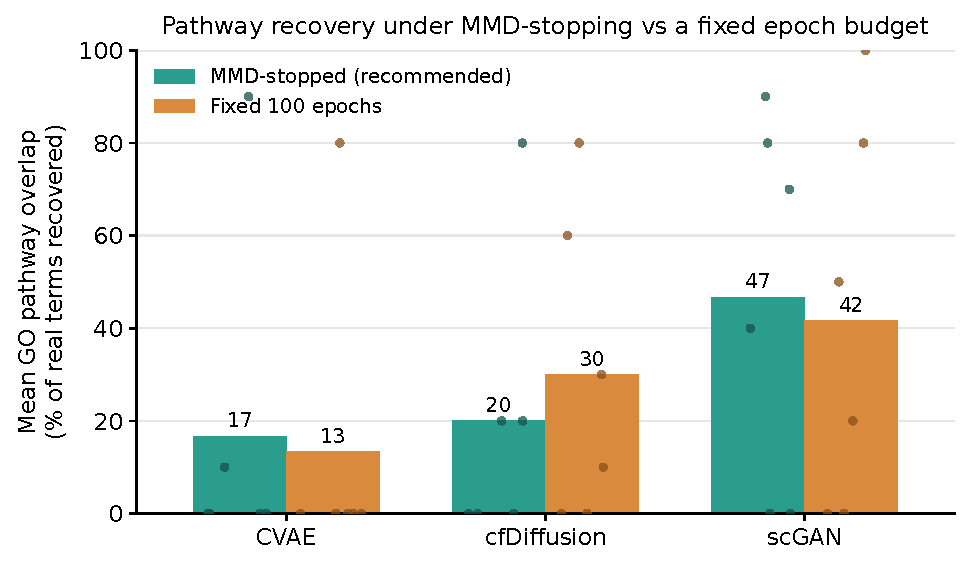
\includegraphics[width=0.72\linewidth]{fig_mmd_stopping.pdf}
\caption{\textbf{MMD-based stopping versus a fixed epoch budget.} Mean gene-ontology pathway overlap (percentage of the real data's enriched terms recovered) for each generator when stopped on MMD (recommended) versus trained for a fixed 100 epochs; dots are the six individual datasets. MMD-stopping improves recovery for the two strongest-conditioned generators (scGAN and CVAE) and avoids the architecture-unfairness of a fixed budget, which raised cfDiffusion on the two largest cohorts while leaving overall recovery comparable (about 28\% either way). The pipeline supports both modes.}
\label{fig:mmdstop}
\end{figure}

\subsection{The sparsity gap constrains latent-space generators}
Real single-cell matrices carried 88 to 98\% zero entries, and the generators diverged sharply in reproducing this dropout structure (Fig.~\ref{fig:sparsity}). The multi-conditional scGAN, which normalizes library size directly in gene space, reproduced near-real sparsity (77 to 97\% zeros), whereas the two latent-space generators under-represented dropout severely: the CVAE produced only 14 to 44\% zeros and cfDiffusion only 16 to 29\%, with cfDiffusion densest on most datasets and the CVAE denser still on OSDR-402 and the cancer control (the single densest matrix in the study). This over-densification follows from generating in a compressed latent space that discards fine-grained zero structure. The practical consequence is that the CVAE and cfDiffusion outputs are presently suited to bulk-like and pathway-level analyses rather than to tasks that depend on accurate dropout, such as cell-type identification and trajectory inference, whereas scGAN's output is closer to usable at single-cell resolution. Sparsity-aware objectives, dropout-preserving latent variables analogous to library-size modeling in scVI \cite{scvi}, or count-based likelihoods are natural next steps for the latent-space models.

\begin{figure}[ht]
\centering
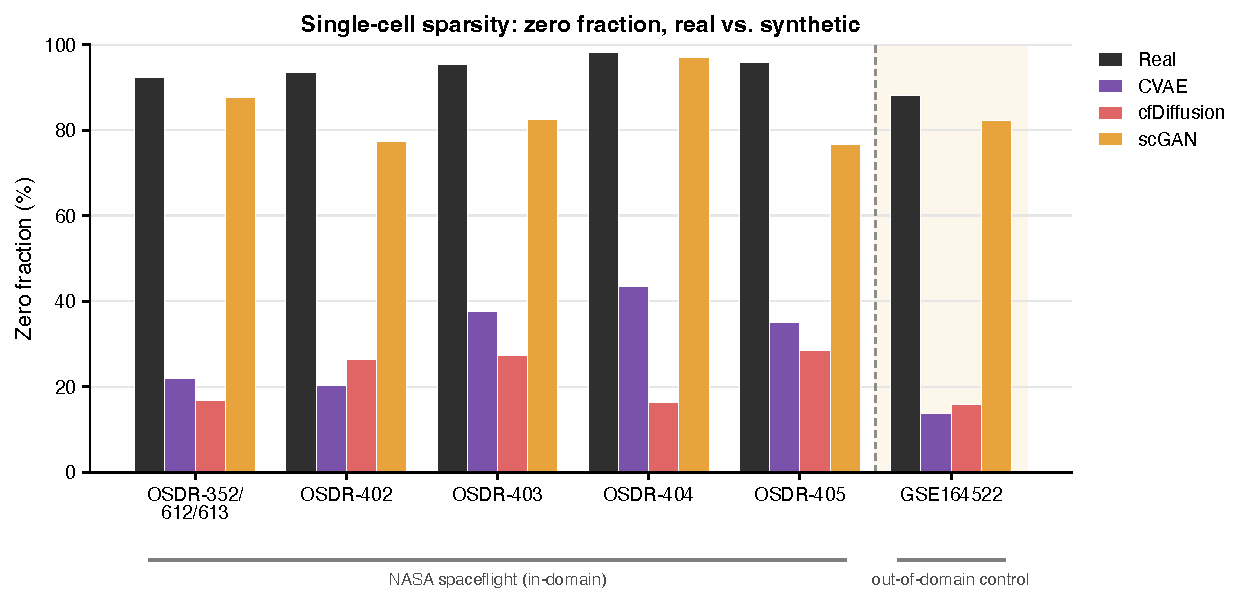
\includegraphics[width=0.92\linewidth]{fig_sparsity.pdf}
\caption{\textbf{Preservation of single-cell sparsity.} Per-matrix zero fraction for real data and for each generator across the panel; the shaded column and bracket labels mark the out-of-domain cancer control against the in-domain spaceflight datasets. scGAN approximates real sparsity closely, while the CVAE and cfDiffusion produce much denser-than-real output, with cfDiffusion densest on most datasets.}
\label{fig:sparsity}
\end{figure}
\FloatBarrier

\subsection{A shared resource for the field}
Beyond the specific results, \fides{} is intended as a community resource. It is accessible, scalable, and model-agnostic, holds every generator to a common MMD operating point and retains the Layer~0 statistical distances so runs stay comparable, and reduces the evaluation of a new generator to running one pipeline rather than re-implementing an ad hoc protocol. As new architectures arrive, this gives the field a consistent basis for deciding which synthetic data preserves the biology, and a fair basis for choosing among generators.

\subsection{Limitations}
Several limitations bound our claims. The dataset panel, while at or above the size used by comparable methods papers \cite{cfgen,scdiffusion,cfdiffusion}, remains modest, and the individual RRRM-2 studies are small, so we report the spread of metrics across datasets rather than single point estimates; two low-signal studies (OSDR-403, OSDR-405) recovered little pathway overlap for any model, consistent with the strong dependence of fidelity on cell count (Fig.~\ref{fig:size}). The complementary per-gene distance metrics and formal significance testing were not computed in this run and are left for future work; we lead with feature-importance overlap rather than TSTR accuracy because the latter dissociates from gene-level fidelity. The multi-conditional adaptations of cfDiffusion and scGAN enable a fair, like-for-like comparison but are not themselves modeling contributions. Finally, predictive-gene enrichment overlap is a new synthetic-data metric and would benefit from further validation against held-out biological-signal recovery. We view establishing this methodological foundation as timely, given that larger spaceflight single-cell datasets are only now becoming available.

\subsection{Implications for spaceflight medicine}
Condition-controllable synthetic cells enable in silico cohorts that are impossible to collect from astronauts, supporting power analyses, countermeasure screening across genetic backgrounds, and the development of predictive health models under the sample scarcity that defines this field \cite{scott,ilangovan}. The multi-conditional generation demonstrated here is what makes such cohorts possible, and \fides{} gives the community a way to decide which synthetic data is trustworthy enough to use for these purposes.

% =====================================================================
\section{Methods}

\subsection{Datasets and preprocessing}
Spaceflight scRNA-seq datasets were obtained from NASA OSDR and evaluated as five configurations: the individual Rodent Research Reference Mission-2 (RRRM-2) studies OSDR-402 (femur bone marrow), OSDR-403 (humerus bone marrow), OSDR-404 (peripheral blood mononuclear cells), and OSDR-405 (spleen), all from female C57BL/6NTac mice, together with one pooled brain cohort combining OSDR-352, OSDR-612, and OSDR-613 across three strains (Table~\ref{tab:data}). One out-of-domain control, the human colorectal-cancer liver-metastasis tumor-immune atlas GSE164522, was processed identically as a robustness check. Count matrices were library-size normalized to $10^4$ and log$(x+1)$ transformed. Genes expressed in a vanishingly small fraction of cells were removed at a 0.997 sparsity threshold ($3\sigma$ cutoff), and the top 2000 highly variable genes were selected \cite{seurat}. Each dataset was split into training, validation, and held-out test partitions stratified by the primary condition; all biological-fidelity metrics were computed on held-out test data to avoid optimistic assessment.

\subsection{Phenotype contrast shared across layers}
A single binary phenotype contrast defines Layers~1 to~3. For the OSDR datasets the two classes are spaceflight and ground control; for the cancer control they are metastatic-site tumor and adjacent normal tissue. These same two classes are the groups compared for differential expression (Layer~1), the labels the random-forest classifier is trained to separate (Layer~2), and the basis for the gene-ontology analysis of the classifier's predictive genes (Layer~3). Using one contrast throughout makes the three biological scores interrogate the same biology and be directly comparable.

\subsection{Shared conditioning vector}
All three generators conditioned on an identical covariate vector, so that the biological comparison reflects the generated data and not differences in conditioning power. For the spaceflight datasets this vector comprised experimental condition (flight versus ground control), biological strain, sex, age at launch, and mission duration; for the cancer control it comprised the major cell-type annotation and tissue compartment. Categorical variables were one-hot encoded and continuous variables were normalized to $[-1,1]$, and the same encoded vector was supplied to every model. This symmetry removes conditioning power as a confounder across the testbed. Because the original cfDiffusion and scGAN implementations condition on a single attribute, we extended both to accept this full multi-attribute vector (below).

\subsection{Conditional variational autoencoder}
The CVAE maps 2000-gene expression vectors to a 32-dimensional latent space through fully connected layers of width $800$ and $400$ with batch normalization, dropout ($0.03$), and nonlinear activations, with the conditioning vector concatenated to the input and again to the latent code before decoding. It maximizes the conditional evidence lower bound,
\begin{equation}
\mathcal{L}_{\mathrm{CVAE}} = \mathbb{E}_{q_\phi(z\mid x,c)}\left[\log p_\theta(x\mid z,c)\right] - \beta\, D_{\mathrm{KL}}\!\left(q_\phi(z\mid x,c)\,\|\,p(z)\right),
\end{equation}
with a Gaussian posterior $q_\phi(z\mid x,c)=\mathcal{N}(z;\mu_\phi(x,c),\sigma_\phi^2(x,c))$, the reparameterization trick for differentiable sampling, a reconstruction term appropriate for normalized expression, and $\beta=0.05$ controlling the Kullback-Leibler regularization. Trained with Adam (learning rate $10^{-2}$, weight decay $10^{-3}$, batch size $128$) in PyTorch.

\subsection{Classifier-free latent diffusion (cfDiffusion)}
Following cfDiffusion \cite{cfdiffusion}, a first-stage variational autoencoder compresses the 2000-gene vectors to a 128-dimensional latent space (encoder $1024\to1024\to128$, decoder reversed; $\beta=10^{-3}$), and a second-stage denoising diffusion model operates in that latent space using a skip-connected network with hidden widths $512,512,256,128$. The forward process adds Gaussian noise over $T=1000$ steps with a cosine schedule $\{\beta_t\}$, $q(z_t\mid z_{t-1})=\mathcal{N}(z_t;\sqrt{1-\beta_t}\,z_{t-1},\beta_t I)$, and the network $\epsilon_\theta(z_t,t,c)$ learns to predict the added noise by minimizing
\begin{equation}
\mathcal{L}_{\mathrm{diff}} = \mathbb{E}_{z_0,c,t,\epsilon}\left[\left\|\epsilon - \epsilon_\theta\!\left(\sqrt{\bar\alpha_t}\,z_0 + \sqrt{1-\bar\alpha_t}\,\epsilon,\; t,\; c\right)\right\|^2\right].
\end{equation}
Classifier-free guidance is enabled by dropping the condition with probability $p_{\mathrm{drop}}=0.1$ during training and combining conditional and unconditional predictions at inference with guidance strength $\gamma=2.0$, $\tilde\epsilon_\theta = \epsilon_\theta(z_t,t,\varnothing) + \gamma\left(\epsilon_\theta(z_t,t,c)-\epsilon_\theta(z_t,t,\varnothing)\right)$. We extended the original single-attribute conditioning to the full multi-attribute vector with a per-attribute embedder bank: each categorical attribute is one-hot encoded and linearly projected and each continuous attribute is linearly projected, each to $128/K$ dimensions for $K$ conditioning attributes; the per-attribute embeddings are concatenated and passed through a linear layer, a nonlinearity, and layer normalization to a single 128-dimensional joint condition embedding. This embedding is injected additively into every residual block alongside the timestep embedding, and under classifier-free dropout (or when an attribute is absent) the corresponding embedding is set to zero, so dropped attributes contribute nothing. Implemented in PyTorch.

\subsection{Multi-conditional scGAN}
The GAN arm is the scGAN architecture of Marouf et al.\ \cite{scgan}, a Wasserstein GAN with gradient penalty and a library-size normalization layer, implemented in TensorFlow. The generator maps a 128-dimensional noise vector through hidden widths $256,512,1024$ to 2000 genes, and the critic mirrors this. The original conditional variant conditions on a single categorical variable (cell type). We extended it to accept the full multi-attribute conditioning vector used by the other two generators by injecting the covariates through conditional (feature-wise) batch normalization: the concatenated condition vector (one-hot categorical plus $[-1,1]$-normalized continuous attributes) is mapped by a small multilayer perceptron to per-layer scale and offset parameters $(\gamma,\beta)$ that modulate each hidden layer's batch-normalized activations in both the generator and the critic, so that generation is controllable on condition, strain, sex, age, and duration jointly. This adaptation lets scGAN accept the same conditioning vector as the CVAE and cfDiffusion; it is a means to a fair comparison rather than a modeling contribution. Trained with Adam ($\beta_1=0$, $\beta_2=0.9$, learning rate $1.5\times10^{-4}$ for both generator and critic), gradient-penalty weight $\lambda_{\mathrm{gp}}=15$, four critic updates per generator update, gradient-norm clipping at $1.0$, and batch size $32$.

\subsection{Training and MMD-based stopping rule}
Training and MMD sampling were class-balanced across all conditions, so that neither the optimization nor the stopping criterion was biased by condition imbalance. Because evidence-lower-bound, adversarial, and denoising losses are not comparable across families, and the adversarial loss in particular does not track sample quality, we trained and stopped all models on a shared external criterion. We fit a 50-component principal-component analysis once on the real training data only and froze it; it was never refit on synthetic or pooled data, which would make MMD non-comparable across models and checkpoints. We drew a single real reference sample of 10{,}000 cells, class-balanced to match the real data, once at the start and reused it unchanged for every evaluation. At each evaluation during training, the model generated a fresh synthetic sample of 10{,}000 cells with the same class balance; both the fixed real reference and the fresh synthetic sample were projected through the frozen PCA, and MMD was computed between the two projections with a radial-basis-function kernel \cite{gretton,sutherland}. The kernel bandwidth was set by the median heuristic on the training data. MMD was never computed in the raw high-dimensional space, where distance concentration renders the kernel insensitive. Training continued while MMD improved and stopped when it ceased to improve over a fixed window, giving each generator its own converged operating point. Using MMD as a shared stopping criterion, so that generators of different families reach a common distributional operating point rather than being halted on incommensurable losses, is a deliberate design choice that makes the biological comparison fair. MMD convergence is treated as a fair common operating point, not as proof that the biology has been fully learned.

\subsection{Biological-fidelity layers}
For every dataset and architecture we generated a full one-to-one replicate of the real dataset, matching the exact distribution of mission parameters (the same combinations of condition, strain, sex, age, and duration), and computed the three biological layers on held-out test data under the train-on-synthetic, test-on-real (TSTR) design: each quantity is derived from synthetic data and scored against the same quantity derived from real held-out data.

\noindent\textbf{Layer 1, condition fidelity (DEG overlap).} Differential expression between the two phenotype classes was computed by t-test separately in real and synthetic data, genes were ranked by absolute (unsigned) log fold change, and the overlap of the top 50 genes was quantified. The value $N=50$ is a convention; the metric is defined for any $N$.

\noindent\textbf{Layer 2, phenotypic fidelity (RF feature-importance overlap, TSTR).} Random-forest classifiers (100 trees, maximum depth 10, five-fold cross-validation repeated three times, i.e.\ 15 fits) were trained to distinguish the two phenotype classes, one on synthetic data and one on real data, using the 2000 highly variable genes as features. Genes were ranked by mean Gini importance across the 15 fits, and the top 50 were compared by overlap. This inverts the classifier two-sample test of prior work \cite{scgan,scdiffusion,lopezpaz}, in which chance-level discrimination is optimal; here, high agreement is optimal. The classifier's accuracy on real held-out cells (TSTR accuracy) is reported as a secondary diagnostic only, because it dissociated from gene-level overlap (notably for the CVAE); it is not a synthetic-versus-real discrimination test.

\noindent\textbf{Layer 3, mechanistic fidelity (GO enrichment of the Layer-2 genes).} The same top-50 random-forest genes from Layer~2 were tested for gene-ontology over-representation with \texttt{gseapy} \cite{gseapy} using a hypergeometric test against the MSigDB ontology collections \cite{msigdb} (the full M5 set for mouse, comprising GO:BP, GO:CC, GO:MF and the Mammalian Phenotype Ontology, with gene universe $N=46{,}339$; and the equivalent C5 set for human, $N=43{,}841$), keeping terms at FDR $q<0.05$ and retaining the top ten by $q$-value. Mechanistic fidelity is the directional percentage of the real data's top enriched terms that the synthetic data also recovers. Because the gene set is the classifier's own predictive genes, this captures functional coherence that gene-level overlap can miss while tying the mechanistic test directly to the phenotypic one.

\subsection{Layer 0: statistical-distance battery}
The Layer~0 statistical layer comprises distributional and per-gene distances between real and synthetic data: cosine distance, Sinkhorn-approximated Wasserstein distance, mean absolute deviation of per-gene means, and pooled-covariance Mahalanobis distance. These distances, and formal significance testing, were not computed in the reported pipeline run and are left for future work; the MMD operating point reached during training (frozen PCA-50) is reported in their place as the statistical anchor at which the architectures are compared (Table~\ref{tab:stat}).

\subsection{Training and hardware}
All models used Adam optimization with the MMD stopping rule above (learning rate $10^{-2}$ for the CVAE, $10^{-3}$ for the cfDiffusion first-stage VAE, and $1.5\times10^{-4}$ for scGAN). Classifier-free guidance used strength $\gamma=2.0$ with condition-drop probability $0.1$; the gradient-penalty weight was $15$ with four critic updates per generator update. Converged operating points occurred at different epochs per model and dataset (Fig.~\ref{fig:mmd}; Table~\ref{tab:stat}). For evaluation, each model generated a one-to-one synthetic replicate of the corresponding real dataset; diffusion sampling used DDIM with \res{number} steps.

\subsection{Code and data availability}
All scRNA-seq datasets are available in the NASA OSDR \cite{osdr} and, for the cancer control, in GEO under accession GSE164522. Training scripts, trained models, generated data, and the \fides{} implementation are available at \res{repository URL}.

% =====================================================================
\section*{Acknowledgements}
We thank the Space Life Sciences Training Program and the AI4LS team at NASA Ames Research Center for support. \res{Add grant numbers, VIP program acknowledgement, and any additional personnel.}

\section*{Author contributions}
\res{Specify, e.g.: A.S.\ conceived the study, implemented the models and the \fides{} framework, ran experiments, and wrote the manuscript; W.A.\ and J.C.\ supervised and edited.}

\section*{Competing interests}
The authors declare no competing interests.

% =====================================================================
\begin{thebibliography}{99}
\small
\bibitem{twins} Garrett-Bakelman FE, et al. The NASA Twins Study: a multidimensional analysis of a year-long human spaceflight. \textit{Science} 364, eaau8650 (2019). doi:10.1126/science.aau8650.
\bibitem{i4} Overbey EG, et al. Spatial and single-cell profiling of the multiomic response to spaceflight. \textit{Nat.\ Commun.} 15, 4954 (2024). doi:10.1038/s41467-024-48916-8.
\bibitem{ilangovan} Ilangovan V, et al. Machine learning classification of spaceflown versus ground-control mice from harmonized liver transcriptomes. \textit{npj Microgravity} 10, 61 (2024). doi:10.1038/s41526-024-00379-3.
\bibitem{scott} Scott RT, Sanders LM, Antonsen EL, et al. Biomonitoring and precision health in deep space supported by artificial intelligence. \textit{Nat.\ Mach.\ Intell.} 5, 196--207 (2023). doi:10.1038/s42256-023-00618-4.
\bibitem{osdr} Gebre SG, et al. NASA Open Science Data Repository: open science for life in space. \textit{Nucleic Acids Res.} 53, D1697--D1710 (2024). doi:10.1093/nar/gkae1116.
\bibitem{scvi} Lopez R, Regier J, Cole MB, Jordan MI, Yosef N. Deep generative modeling for single-cell transcriptomics. \textit{Nat.\ Methods} 15, 1053--1058 (2018). doi:10.1038/s41592-018-0229-2.
\bibitem{activa} Heydari AA, Davalos OA, Zhao L, Hoyer KK, Sindi SS. ACTIVA: realistic single-cell RNA-seq generation with automatic cell-type identification using introspective variational autoencoders. \textit{Bioinformatics} 38, 2194--2201 (2022). doi:10.1093/bioinformatics/btac095.
\bibitem{scgan} Marouf M, et al. Realistic in silico generation and augmentation of single-cell RNA-seq data using generative adversarial networks. \textit{Nat.\ Commun.} 11, 166 (2020). doi:10.1038/s41467-019-14018-z.
\bibitem{scdiffusion} Luo E, Hao M, Wei L, Zhang X. scDiffusion: conditional generation of high-quality single-cell data using diffusion model. \textit{Bioinformatics} 40, btae518 (2024). doi:10.1093/bioinformatics/btae518.
\bibitem{cfdiffusion} Zhang T, Zhao Z, Ren J, Zhang Z, Zhang H, Wang G. cfDiffusion: diffusion-based efficient generation of high-quality scRNA-seq data with classifier-free guidance. \textit{Brief.\ Bioinform.} 26, bbaf071 (2025). doi:10.1093/bib/bbaf071.
\bibitem{cfgen} Palma A, et al. Multi-modal and multi-attribute generation of single cells with CFGen. \textit{Proc.\ ICLR} (2025). arXiv:2407.11734.
\bibitem{scgft} Tedesco M, et al. Single-cell generative modeling with the Fourier transform (scGFT). \textit{Commun.\ Biol.} 8, 1 (2025). doi:10.1038/s42003-025-07552-8.
\bibitem{scdesign3} Song D, et al. scDesign3 generates realistic in silico data for multimodal single-cell and spatial omics. \textit{Nat.\ Biotechnol.} 41, 1610--1618 (2023). doi:10.1038/s41587-023-01772-1.
\bibitem{simbench} Cao Y, Yang P, Yang JYH. A benchmark study of simulation methods for single-cell RNA sequencing data. \textit{Nat.\ Commun.} 12, 6911 (2021). doi:10.1038/s41467-021-27130-w.
\bibitem{gretton} Gretton A, Borgwardt KM, Rasch MJ, Sch\"olkopf B, Smola A. A kernel two-sample test. \textit{J.\ Mach.\ Learn.\ Res.} 13, 723--773 (2012).
\bibitem{sutherland} Sutherland DJ, et al. Generative models and model criticism via optimized maximum mean discrepancy. \textit{Proc.\ ICLR} (2017). arXiv:1611.04488.
\bibitem{gseapy} Fang Z, Liu X, Peltz G. GSEApy: a comprehensive package for performing gene set enrichment analysis in Python. \textit{Bioinformatics} 39, btac757 (2023). doi:10.1093/bioinformatics/btac757.
\bibitem{msigdb} Liberzon A, Birger C, Thorvaldsd\'ottir H, Ghandi M, Mesirov JP, Tamayo P. The Molecular Signatures Database (MSigDB) hallmark gene set collection. \textit{Cell Syst.} 1, 417--425 (2015). doi:10.1016/j.cels.2015.12.004.
\bibitem{esteban} Esteban C, Hyland SL, R\"atsch G. Real-valued (medical) time series generation with recurrent conditional GANs. \textit{arXiv} 1706.02633 (2017).
\bibitem{lopezpaz} Lopez-Paz D, Oquab M. Revisiting classifier two-sample tests. \textit{Proc.\ ICLR} (2017). arXiv:1610.06545.
\bibitem{seurat} Hafemeister C, Satija R. Normalization and variance stabilization of single-cell RNA-seq data using regularized negative binomial regression. \textit{Genome Biol.} 20, 296 (2019). doi:10.1186/s13059-019-1874-1.
\bibitem{tenx} Zheng GXY, et al. Massively parallel digital transcriptional profiling of single cells. \textit{Nat.\ Commun.} 8, 14049 (2017). doi:10.1038/ncomms14049.
\bibitem{ntrs} Golts A, Casaletto J, Costes SV. \res{Conditional variational autoencoder for spaceflight single-nucleus RNA-seq (poster title to confirm).} NASA Technical Reports Server (NTRS) (2024).
\bibitem{glare} \res{Authors to confirm.} GLARE: augmentation framework for spaceflight omics. \textit{npj Microgravity} (2025). doi:10.1038/s41526-025-00525-5.
\bibitem{ganbio} \res{Authors to confirm.} Generative adversarial networks for biomarker discovery from NASA OSDR transcriptomes. \textit{Neuroinformatics} (2025). doi:10.1007/s12021-025-09729-2.
\end{thebibliography}

\end{document}
